\documentclass{standalone}
\usepackage{tikz}
\usetikzlibrary{patterns, positioning}


\begin{document}
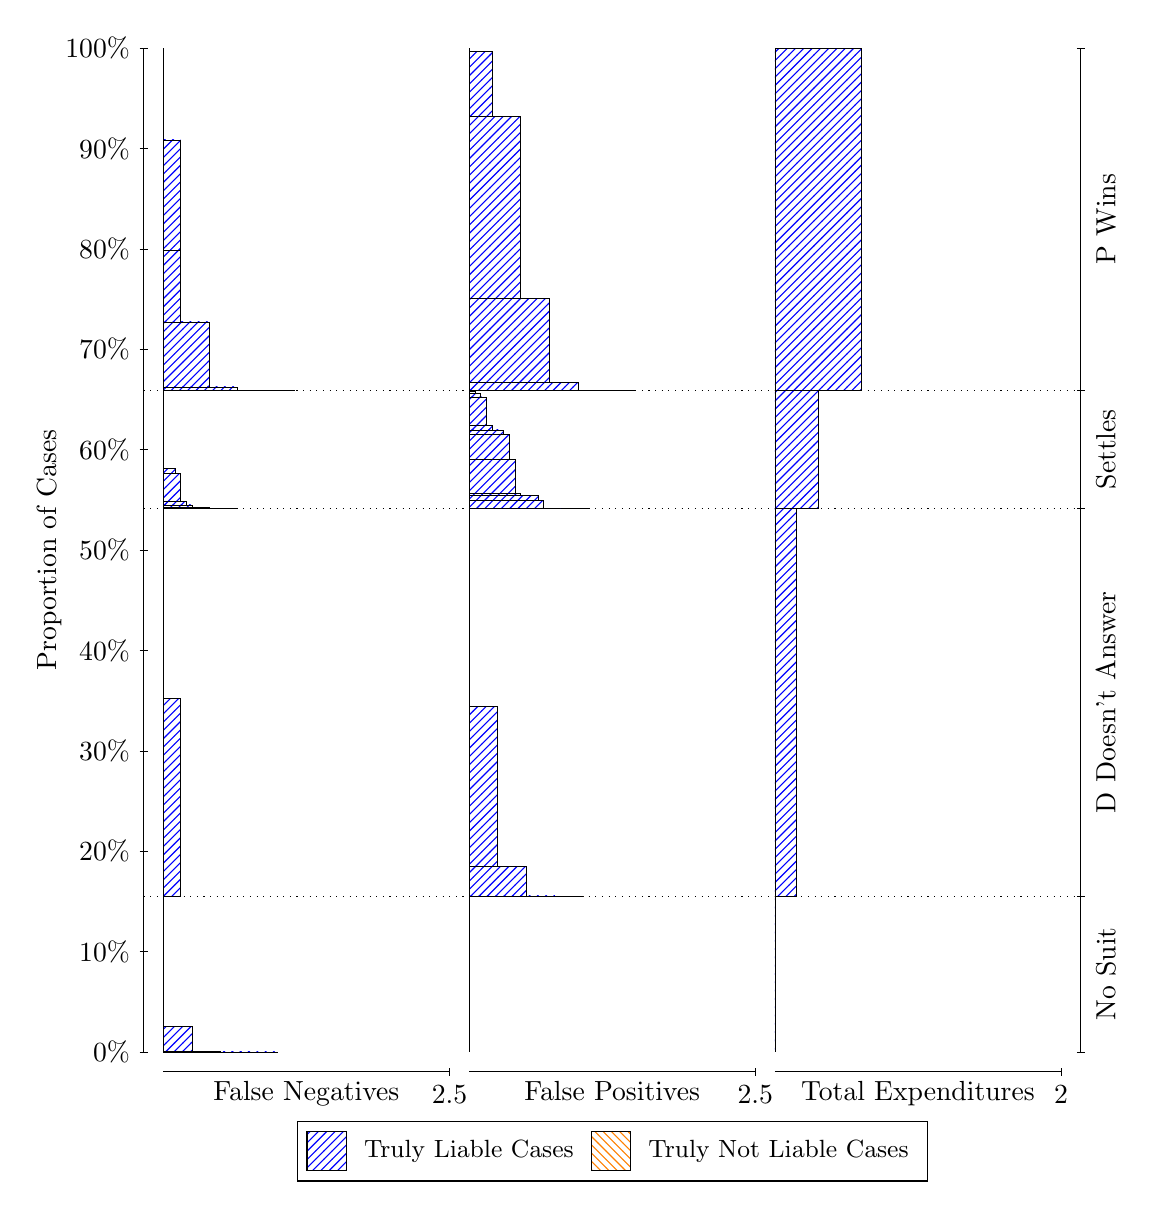
\begin{tikzpicture}
\draw[black, very thin] (1.5,1.75) -- (1.5,14.5);
\node[rotate=90, text=black, anchor=center] at (0.3, 8.125) {Proportion of Cases};
\draw[black, very thin] (1.45,1.75) -- (1.55,1.75);
\node[text=black, anchor=east] at (1.45, 1.75) {0\%};
\draw[black, very thin] (1.45,3.025) -- (1.55,3.025);
\node[text=black, anchor=east] at (1.45, 3.025) {10\%};
\draw[black, very thin] (1.45,4.3) -- (1.55,4.3);
\node[text=black, anchor=east] at (1.45, 4.3) {20\%};
\draw[black, very thin] (1.45,5.575) -- (1.55,5.575);
\node[text=black, anchor=east] at (1.45, 5.575) {30\%};
\draw[black, very thin] (1.45,6.85) -- (1.55,6.85);
\node[text=black, anchor=east] at (1.45, 6.85) {40\%};
\draw[black, very thin] (1.45,8.125) -- (1.55,8.125);
\node[text=black, anchor=east] at (1.45, 8.125) {50\%};
\draw[black, very thin] (1.45,9.4) -- (1.55,9.4);
\node[text=black, anchor=east] at (1.45, 9.4) {60\%};
\draw[black, very thin] (1.45,10.675) -- (1.55,10.675);
\node[text=black, anchor=east] at (1.45, 10.675) {70\%};
\draw[black, very thin] (1.45,11.95) -- (1.55,11.95);
\node[text=black, anchor=east] at (1.45, 11.95) {80\%};
\draw[black, very thin] (1.45,13.225) -- (1.55,13.225);
\node[text=black, anchor=east] at (1.45, 13.225) {90\%};
\draw[black, very thin] (1.45,14.5) -- (1.55,14.5);
\node[text=black, anchor=east] at (1.45, 14.5) {100\%};

\draw[black, very thin] (13.4,1.75) -- (13.4,14.5);
\draw[black, very thin] (13.35,1.75) -- (13.45,1.75);
\node[anchor=west] at (13.35, 1.75) {};
\draw[black, very thin] (13.35,3.7294) -- (13.45,3.7294);
\node[anchor=west] at (13.35, 3.7294) {};
\draw[black, very thin] (13.35,8.6542) -- (13.45,8.6542);
\node[anchor=west] at (13.35, 8.6542) {};
\draw[black, very thin] (13.35,10.155) -- (13.45,10.155);
\node[anchor=west] at (13.35, 10.155) {};
\draw[black, very thin] (13.35,14.5) -- (13.45,14.5);
\node[anchor=west] at (13.35, 14.5) {};

\draw[black, very thin, pattern color=blue, pattern=north east lines] (1.75,1.75) rectangle (3.2033,1.75);
\draw[black, very thin, pattern color=blue, pattern=north east lines] (1.75,1.75) rectangle (2.84,1.75);
\draw[black, very thin, pattern color=blue, pattern=north east lines] (1.75,1.75) rectangle (2.4767,1.7528);
\draw[black, very thin, pattern color=blue, pattern=north east lines] (1.75,1.7528) rectangle (2.1133,2.0741);
\draw[black, very thin, pattern color=orange, pattern=north west lines] (1.75,2.0741) rectangle (1.75,2.0741);
\draw[black, very thin, pattern color=blue, pattern=north east lines] (1.75,2.0741) rectangle (1.75,3.7294);
\draw[black, very thin, pattern color=blue, pattern=north east lines] (1.75,3.7294) rectangle (1.968,6.2438);
\draw[black, very thin, pattern color=orange, pattern=north west lines] (1.75,6.2438) rectangle (1.75,6.2438);
\draw[black, very thin, pattern color=blue, pattern=north east lines] (1.75,6.2438) rectangle (1.75,8.6542);
\draw[black, very thin, pattern color=blue, pattern=north east lines] (1.75,8.6542) rectangle (2.6947,8.6542);
\draw[black, very thin, pattern color=blue, pattern=north east lines] (1.75,8.6542) rectangle (2.404,8.6542);
\draw[black, very thin, pattern color=blue, pattern=north east lines] (1.75,8.6542) rectangle (2.3313,8.6671);
\draw[black, very thin, pattern color=blue, pattern=north east lines] (1.75,8.6671) rectangle (2.2587,8.6702);
\draw[black, very thin, pattern color=blue, pattern=north east lines] (1.75,8.6702) rectangle (2.1133,8.6986);
\draw[black, very thin, pattern color=blue, pattern=north east lines] (1.75,8.6986) rectangle (2.0407,8.7397);
\draw[black, very thin, pattern color=blue, pattern=north east lines] (1.75,8.7397) rectangle (1.968,9.1001);
\draw[black, very thin, pattern color=blue, pattern=north east lines] (1.75,9.1001) rectangle (1.8953,9.159);
\draw[black, very thin, pattern color=orange, pattern=north west lines] (1.75,9.159) rectangle (1.75,9.159);
\draw[black, very thin, pattern color=blue, pattern=north east lines] (1.75,9.159) rectangle (1.75,10.155);
\draw[black, very thin, pattern color=blue, pattern=north east lines] (1.75,10.155) rectangle (3.4213,10.155);
\draw[black, very thin, pattern color=blue, pattern=north east lines] (1.75,10.155) rectangle (3.058,10.155);
\draw[black, very thin, pattern color=blue, pattern=north east lines] (1.75,10.155) rectangle (2.6947,10.196);
\draw[black, very thin, pattern color=blue, pattern=north east lines] (1.75,10.196) rectangle (2.3313,11.022);
\draw[black, very thin, pattern color=blue, pattern=north east lines] (1.75,11.022) rectangle (1.968,11.927);
\draw[black, very thin, pattern color=blue, pattern=north east lines] (1.75,11.927) rectangle (1.968,13.332);
\draw[black, very thin, pattern color=orange, pattern=north west lines] (1.75,13.332) rectangle (1.75,13.332);
\draw[black, very thin, pattern color=blue, pattern=north east lines] (1.75,13.332) rectangle (1.75,14.5);
\draw[black, very thin, pattern color=orange, pattern=north west lines] (5.6333,1.75) rectangle (5.6333,1.75);
\draw[black, very thin, pattern color=blue, pattern=north east lines] (5.6333,1.75) rectangle (5.6333,3.7294);
\draw[black, very thin, pattern color=orange, pattern=north west lines] (5.6333,3.7294) rectangle (7.0867,3.7294);
\draw[black, very thin, pattern color=blue, pattern=north east lines] (5.6333,3.7294) rectangle (7.0867,3.7294);
\draw[black, very thin, pattern color=blue, pattern=north east lines] (5.6333,3.7294) rectangle (6.7233,3.7322);
\draw[black, very thin, pattern color=blue, pattern=north east lines] (5.6333,3.7322) rectangle (6.36,4.1099);
\draw[black, very thin, pattern color=blue, pattern=north east lines] (5.6333,4.1099) rectangle (5.9967,6.1398);
\draw[black, very thin, pattern color=blue, pattern=north east lines] (5.6333,6.1398) rectangle (5.6333,8.6542);
\draw[black, very thin, pattern color=orange, pattern=north west lines] (5.6333,8.6542) rectangle (7.1593,8.6542);
\draw[black, very thin, pattern color=blue, pattern=north east lines] (5.6333,8.6542) rectangle (7.1593,8.6542);
\draw[black, very thin, pattern color=orange, pattern=north west lines] (5.6333,8.6542) rectangle (7.014,8.6542);
\draw[black, very thin, pattern color=blue, pattern=north east lines] (5.6333,8.6542) rectangle (7.014,8.6542);
\draw[black, very thin, pattern color=orange, pattern=north west lines] (5.6333,8.6542) rectangle (6.8687,8.6542);
\draw[black, very thin, pattern color=blue, pattern=north east lines] (5.6333,8.6542) rectangle (6.8687,8.6543);
\draw[black, very thin, pattern color=blue, pattern=north east lines] (5.6333,8.6543) rectangle (6.796,8.6543);
\draw[black, very thin, pattern color=blue, pattern=north east lines] (5.6333,8.6543) rectangle (6.6507,8.6545);
\draw[black, very thin, pattern color=orange, pattern=north west lines] (5.6333,8.6545) rectangle (6.578,8.6545);
\draw[black, very thin, pattern color=blue, pattern=north east lines] (5.6333,8.6545) rectangle (6.578,8.7507);
\draw[black, very thin, pattern color=blue, pattern=north east lines] (5.6333,8.7507) rectangle (6.5053,8.8183);
\draw[black, very thin, pattern color=blue, pattern=north east lines] (5.6333,8.8183) rectangle (6.4327,8.8204);
\draw[black, very thin, pattern color=blue, pattern=north east lines] (5.6333,8.8204) rectangle (6.2873,8.8447);
\draw[black, very thin, pattern color=blue, pattern=north east lines] (5.6333,8.8447) rectangle (6.2147,9.2731);
\draw[black, very thin, pattern color=blue, pattern=north east lines] (5.6333,9.2731) rectangle (6.142,9.5939);
\draw[black, very thin, pattern color=blue, pattern=north east lines] (5.6333,9.5939) rectangle (6.0693,9.65);
\draw[black, very thin, pattern color=blue, pattern=north east lines] (5.6333,9.65) rectangle (5.924,9.7089);
\draw[black, very thin, pattern color=blue, pattern=north east lines] (5.6333,9.7089) rectangle (5.8513,10.069);
\draw[black, very thin, pattern color=blue, pattern=north east lines] (5.6333,10.069) rectangle (5.7787,10.111);
\draw[black, very thin, pattern color=blue, pattern=north east lines] (5.6333,10.111) rectangle (5.706,10.139);
\draw[black, very thin, pattern color=blue, pattern=north east lines] (5.6333,10.139) rectangle (5.6333,10.155);
\draw[black, very thin, pattern color=orange, pattern=north west lines] (5.6333,10.155) rectangle (7.7407,10.155);
\draw[black, very thin, pattern color=blue, pattern=north east lines] (5.6333,10.155) rectangle (7.7407,10.155);
\draw[black, very thin, pattern color=orange, pattern=north west lines] (5.6333,10.155) rectangle (7.3773,10.155);
\draw[black, very thin, pattern color=blue, pattern=north east lines] (5.6333,10.155) rectangle (7.3773,10.156);
\draw[black, very thin, pattern color=orange, pattern=north west lines] (5.6333,10.156) rectangle (7.014,10.156);
\draw[black, very thin, pattern color=blue, pattern=north east lines] (5.6333,10.156) rectangle (7.014,10.252);
\draw[black, very thin, pattern color=orange, pattern=north west lines] (5.6333,10.252) rectangle (6.6507,10.252);
\draw[black, very thin, pattern color=blue, pattern=north east lines] (5.6333,10.252) rectangle (6.6507,11.323);
\draw[black, very thin, pattern color=orange, pattern=north west lines] (5.6333,11.323) rectangle (6.2873,11.323);
\draw[black, very thin, pattern color=blue, pattern=north east lines] (5.6333,11.323) rectangle (6.2873,13.632);
\draw[black, very thin, pattern color=blue, pattern=north east lines] (5.6333,13.632) rectangle (5.924,14.459);
\draw[black, very thin, pattern color=blue, pattern=north east lines] (5.6333,14.459) rectangle (5.6333,14.5);
\draw[black, very thin, pattern color=orange, pattern=north west lines] (9.5167,1.75) rectangle (9.5167,1.75);
\draw[black, very thin, pattern color=blue, pattern=north east lines] (9.5167,1.75) rectangle (9.5167,3.7294);
\draw[black, very thin, pattern color=orange, pattern=north west lines] (9.5167,3.7294) rectangle (9.7892,3.7294);
\draw[black, very thin, pattern color=blue, pattern=north east lines] (9.5167,3.7294) rectangle (9.7892,8.6542);
\draw[black, very thin, pattern color=orange, pattern=north west lines] (9.5167,8.6542) rectangle (10.062,8.6542);
\draw[black, very thin, pattern color=blue, pattern=north east lines] (9.5167,8.6542) rectangle (10.062,10.155);
\draw[black, very thin, pattern color=orange, pattern=north west lines] (9.5167,10.155) rectangle (10.607,10.155);
\draw[black, very thin, pattern color=blue, pattern=north east lines] (9.5167,10.155) rectangle (10.607,14.5);
\draw[black, dotted] (1.5,3.7294) -- (13.4,3.7294);
\draw[black, dotted] (1.5,8.6542) -- (13.4,8.6542);
\draw[black, dotted] (1.5,10.155) -- (13.4,10.155);
\draw[black, very thin] (1.75,1.5) -- (5.3833,1.5);
\node[text=black, anchor=north] at (3.5667, 1.5) {False Negatives};
\draw[black, very thin] (5.3833,1.45) -- (5.3833,1.55);
\node[text=black, anchor=north] at (5.3833, 1.45) {2.5};

\draw[black, very thin] (5.6333,1.5) -- (9.2667,1.5);
\node[text=black, anchor=north] at (7.45, 1.5) {False Positives};
\draw[black, very thin] (9.2667,1.45) -- (9.2667,1.55);
\node[text=black, anchor=north] at (9.2667, 1.45) {2.5};

\draw[black, very thin] (9.5167,1.5) -- (13.15,1.5);
\node[text=black, anchor=north] at (11.333, 1.5) {Total Expenditures};
\draw[black, very thin] (13.15,1.45) -- (13.15,1.55);
\node[text=black, anchor=north] at (13.15, 1.45) {2};

\node[text=black, centered, rotate=90] at (13.72, 2.7397) {No Suit};
\node[text=black, centered, rotate=90] at (13.72, 6.1918) {D Doesn't Answer};
\node[text=black, centered, rotate=90] at (13.72, 9.4045) {Settles};
\node[text=black, centered, rotate=90] at (13.72, 12.327) {P Wins};

\draw (7.449999999999999,1.5) node[draw=none] (baseCoordinate) {};
\begin{scope}[align=center]
        \matrix[scale=0.5, draw=black, below=0.5cm of baseCoordinate, nodes={draw}, column sep=0.1cm]{
            \node[rectangle, draw, minimum width=0.5cm, minimum height=0.5cm, pattern color=blue, pattern=north east lines] {}; &
            \node[draw=none, font=\small, text=black] (B) {Truly Liable Cases}; &
            \node[rectangle, draw, minimum width=0.5cm, minimum height=0.5cm, pattern color=orange, pattern=north west lines] {}; &
            \node[draw=none, font=\small, text=black] (B) {Truly Not Liable Cases}; \\
            };
\end{scope}

\end{tikzpicture}
\end{document}